\documentclass[12pt]{article}
\usepackage[english]{babel}

\usepackage[T1]{fontenc}
\usepackage[utf8]{inputenc}
\usepackage{lmodern}

\usepackage{amsmath, amsfonts, amssymb, dsfont, mathrsfs}
\allowdisplaybreaks

\usepackage{placeins}
\usepackage{wrapfig}
\usepackage{caption}

\usepackage{graphicx, adjustbox, float, xcolor}

\usepackage{tikz, pgfplots}
\pgfplotsset{compat=1.17}
\usetikzlibrary{arrows.meta, automata, positioning,
                decorations.pathreplacing, decorations.markings}

\usepackage{booktabs, enumitem, caption}

\usepackage{listings}
\usepackage{inconsolata} 
\usepackage{upquote}    
\usepackage{mathtools}
\definecolor{rstudioBG}{RGB}{250,250,250}
\definecolor{rstudioFrame}{RGB}{220,220,220}
\definecolor{rstudioBlue}{RGB}{0,92,197}  
\definecolor{rstudioGreen}{RGB}{0,128,0}  
\definecolor{rstudioRed}{RGB}{163,21,21}  
\definecolor{rstudioNum}{RGB}{128,0,128}  

\lstdefinelanguage{R}{
  alsoletter={._},
  morekeywords={if,else,repeat,while,function,for,in,next,break,TRUE,FALSE,NA,NaN,Inf,NULL},
  morekeywords={[2]library,require,data,plot,ggplot,geom_point,geom_line,aes,
               summary,lm,glm,anova,predict,confint,print,cat,read.csv,head,
               dplyr,mutate,select,filter,arrange,group_by,summarise,as.factor,
               factor,as.numeric,as.character,seq,rep,mean,median,sd,var,cor},
  sensitive=true
}

\lstdefinestyle{RStudio}{
  language=R,
  basicstyle=\ttfamily\footnotesize,
  backgroundcolor=\color{rstudioBG},
  frame=single,
  framerule=0.4pt,
  rulecolor=\color{rstudioFrame},
  framesep=3pt,
  numbers=left,
  numberstyle=\tiny\color{gray},
  numbersep=8pt,
  showstringspaces=false,
  breaklines=true,
  columns=fullflexible,
  keepspaces=true,
    aboveskip=0.5em,  
  belowskip=1.1em,   
  keywordstyle=\color{rstudioBlue}\bfseries,     
  keywordstyle={[2]\color{rstudioBlue}},      
  commentstyle=\itshape\color{rstudioGreen},
  stringstyle=\color{rstudioRed},
  literate=
    *{0}{{{\color{rstudioNum}0}}}{1}
     {1}{{{\color{rstudioNum}1}}}{1}
     {2}{{{\color{rstudioNum}2}}}{1}
     {3}{{{\color{rstudioNum}3}}}{1}
     {4}{{{\color{rstudioNum}4}}}{1}
     {5}{{{\color{rstudioNum}5}}}{1}
     {6}{{{\color{rstudioNum}6}}}{1}
     {7}{{{\color{rstudioNum}7}}}{1}
     {8}{{{\color{rstudioNum}8}}}{1}
     {9}{{{\color{rstudioNum}9}}}{1},
}

\lstdefinestyle{RStudioNonum}{
  style=RStudio,
  numbers=none,
}

\newcommand{\rinline}[1]{%
  \fcolorbox{rstudioFrame}{rstudioBG}{%
    \lstinline[style=RStudioNonum,breaklines=false]!#1!%
  }%
}

\lstset{style=RStudio}

\usepackage{hyperref}
\hypersetup{
  colorlinks=true,
  linkcolor=blue,
  citecolor=blue,
  urlcolor=blue
}

\usepackage{titlesec}

\titleformat{\section}
  {\normalsize\bfseries}
  {\thesection}{1em}{}

\titleformat{\subsection}
  {\small\bfseries}
  {\thesubsection}{1em}{}

\setlength{\parskip}{-0.8em}  
\setlength{\parindent}{0pt}   

\usepackage[a4paper,
  includehead,
  margin=20mm,
   top=5mm,
   bottom=20mm
]{geometry}

\usepackage{fancyhdr}
\pagestyle{fancy}
\lhead{Ben Vickers - 304024}
\rhead{Linear Statistical Models - Project}
\setlength{\headsep}{1cm}
\newcommand{\plusorstar}{\ensuremath{\mathbin{\substack{+\\[-0.2ex]*}}}}

\newcommand{\R}{\textsf{R}}

\title{Ben Vickers - 304024 - Reaction Times Project}
\author{} 
\date{} 

\makeatletter
\renewcommand{\@maketitle}{%
  \newpage
  \null
  \vspace*{-1.55cm}
  \begin{center}
{\fontsize{16}{18}\selectfont\bfseries \@title\par}%
    \vskip 0.2cm 
  \end{center}
}
\makeatother

\begin{document}

\maketitle
\section{SUMMARY}
 This project studied the reaction times of one participant across $3$ sets of $36$ unique tests. A clear linear relationship was found between font size and reaction time, with a $95\%$ confidence interval (CI) of  $(42$,$68)$\textsuperscript{\ref{app:diff_CI}} milliseconds (ms) for the difference between the largest and smallest font sizes. Reactions to black text were $\approx\!14\,$ms slower than to yellow, and $\approx\!23\,$ms slower than to white text, and reactions to green backgrounds were $\approx\!18\,$ms faster than to red backgrounds.\textsuperscript{\ref{app:contrasts}} Overall, larger, high-contrast text (e.g. white/yellow on green) resulted in faster reaction times.\newline


\vspace{-0.5cm}
\section{INTRODUCTION}

We suppose a government must procure new road signs with standard colours of white, yellow, or
black text on red or green backgrounds. We aim to investigate how font size and these road sign
colour combinations affect reaction times. Our initial hypothesis was that larger font sizes, and higher-contrast colour pairs could lead to faster reactions, with the effect of certain colour factors potentially changing (interacting) with font size under particular pairings.
\section{METHOD}


Mean reaction times from 10 odd/even reactions were measured at six font sizes:~$0,2,5,7,10,12$. The $36$ combinations of font size, font colour (Black, White, Yellow) and background colour (Green, Red)
were randomised in Excel using \texttt{RAND()} and tested in $3$ groups (\texttt{block}) of $12$ separated by five minute breaks. This process was repeated on three consecutive days (\texttt{session}) under, insofar as possible, identical conditions, forming a randomised block design (RBD) to account for any nuisance factors, e.g. eyestrain or daily energy. All tests used Arial font, no variability, and 175\% zoom, and any run with an incorrect key pressed when reacting was discarded and immediately repeated. We assume the binary odd/even reactions provide a reasonable model for driving decisions such as reacting to give way/priority signs with similar colours.\newline

Based on Plots~\ref{plot:Plot1} and~\ref{plot:Plot2} (and Figures~\ref{fig:blocksessiontimes} and \ref{fig:interactions}), several multiple regression models were fitted in \textsf{R}. A stepwise regression approach was employed with pairwise model comparison tests (MCT) (performed at a significance level of $\alpha\!=\!5\%$) to assess potential for quadratic, and change-point terms in font size, Box-Cox transformations, and interactions between factors. This process resulted in a main effects model including the session and block nuisance factors: \resizebox{\linewidth}{!}{%
\rinline{MLR_RBD=lm(mean_time~font_size+factor(font_colour)+factor(bg_colour)+factor(session)+factor(block))}} This model was validated by several diagnostic plots\textsuperscript{\ref{app:diagnostics}} and aligned with our experimental design, allowing for variation in performance both between, and during sessions.

\section{ANALYSIS}
\enlargethispage{0cm}
\begin{wrapfigure}[11]{l}{0.37\textwidth} 
\vspace{-0.7cm}  \refstepcounter{figure}\label{plot:Plot1}
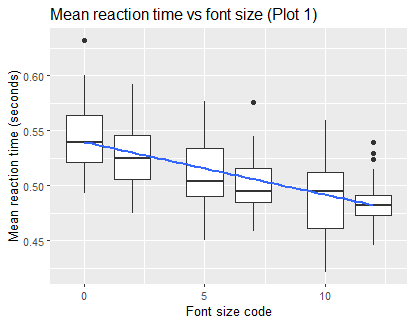
\includegraphics[width=1\linewidth]{Project plots/plot1b.png} 
\vspace{-0.8cm} 
 \end{wrapfigure}

\vspace{0.1cm}A preliminary analysis of the data from Plot~\ref{plot:Plot1} suggested an approximately linear (non-piecewise) relationship between font size and reaction time. Single and multiple main effects regression models gave strong evidence that mean reaction time decreases by $\approx4.8\,$ms per font size code ($p\!=\!1.83\!\cdot\!10^{-10}$).\textsuperscript{\ref{app:simple_effects}} MCTs comparing this simple linear effect with models including quadratic and change-point terms in font size showed no improvement in fit.\textsuperscript{\ref{app:change}, \ref{app:quadratic}} This provides strong support for our first hypothesis that increasing font size improves reaction time.
$ $\newline

\vspace{-0.6cm} \enlargethispage{0cm} From Plot~\ref{plot:Plot2}, we observed that green backgrounds appeared to give faster reactions than red, and white text (and perhaps yellow also) appeared faster than black text. MCTs comparing a model with font size only to models that respectively added font, and background colour main effects, then both, showed that (all allowing for font size) including both font and background colour main effects significantly improved the fit to our data ($p\!=\!8.7\!\cdot\!10^{-4}$).\textsuperscript{\ref{app:simple_effects}} This justified the addition of both colour main effects to subsequent model comparisons.
\newpage
\begin{wrapfigure}[17]{l}{0.37\textwidth} 
  \vspace{-0.6cm}  \refstepcounter{figure}\label{plot:Plot2}
  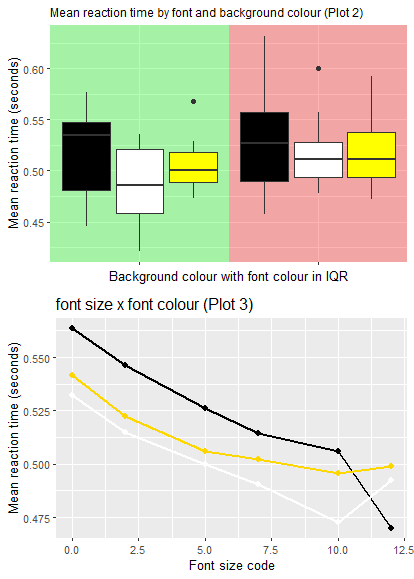
\includegraphics[width=\linewidth]{Project plots/plot2and3.png}
\end{wrapfigure}

\vspace*{-0.1cm} Recalling that prior to our experiment, we expected similar responses on each day and within each group of $12$ tests, mean reaction times were plotted over each of these factors.\textsuperscript{\ref{app:blocking}} Based on this output, we applied an RBD by adding the two nuisance factors to the main effects model which reduced $RSS$ by $\approx\!34.6\%$\textsuperscript{\ref{app:blocking}} and MCTs showed a significantly improved fit over the prior\refstepcounter{figure}\label{plot:Plot3}, non-blocking model ($p\!=\!1.4\cdot10^{-8}$).\textsuperscript{\ref{app:blocking}} This provided strong support for including both nuisance factors instead of proceeding under a completely randomised design model that ignored our expected sources of variation.
\vspace{0.5cm} \par
  Considering the possibility of interaction effects, two-way interaction plots were observed whereby Plot~\ref{plot:Plot3} showed (over a small region) non-parallel lines for \texttt{font\_size}$\times$\texttt{font\_colour}. An MCT comparing \rinline{MLR_RBD} to a model including this interaction term yielded only borderline evidence for its significance ($p\!=\!0.059$) and only a small reduction in $RSS$ of $\approx6\%$.\textsuperscript{\ref{app:interactions}} Therefore, we retained main effects only and concluded that contrary to our hypothesised presence of interactions, no interaction terms between any factor combinations were supported by the experiment's data at a $5\%$ significance level.\newline

Under model \rinline{MLR_RBD}, a linear contrast showed that black font reactions were $\approx 14\,$ms slower than yellow $(p\!=\!0.044$) and $\approx 23\,$ms slower than white $(p\!=\!0.0005)$, whereas, yellow and white fonts were not significantly different ($p\!=\!0.25$).\textsuperscript{\ref{app:contrasts}} It also showed that red background reactions were $\approx 18\,$ms slower than green ($p\!=\!0.0003$),\textsuperscript{\ref{app:model_summary}} hence we have significant evidence to support the first aspect of our second hypothesis that higher contrast combinations (e.g. green backgrounds and white/yellow fonts) yield faster reactions.\newline

\begin{wrapfigure}[7]{l}{0.5\textwidth} 
\vspace{-0.5cm}\refstepcounter{figure}\label{plot:Plot4}\refstepcounter{figure}\label{plot:Plot5}
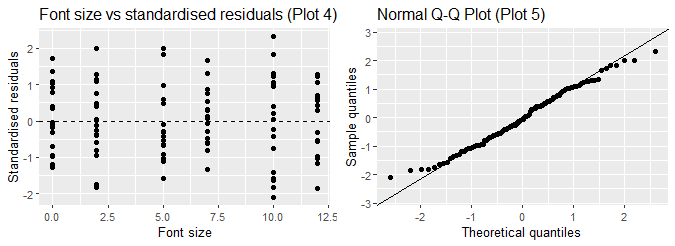
\includegraphics[width=1\linewidth]{Project plots/4and5.png} 
\vspace{-0.8cm}
 \end{wrapfigure}
\par
\noindent

Model diagnostics for \rinline{MLR_RBD} in Plot~\ref{plot:Plot5} show a Q–Q plot with only minor skewing in the tails. Although a Box–Cox transformation suggested $\hat{\lambda} \!=\! -0.1$, its CI was very wide and contained $1$, and diagnostic plots of a $\log$-transformed model showed no improvement.\textsuperscript{\ref{app:boxcox}} Plot~\ref{plot:Plot4} shows standardised residuals of \rinline{MLR_RBD} against font size with no visible patterns and seemingly random scatter, and residuals plotted against both fitted values, and run index, demonstrate similar adherence to normality assumptions, with $\approx 95\%$ of residuals in $(-1.96,1.96)$.\textsuperscript{\ref{app:diagnostics}} Therefore, given the reasonably small sample size, we accept the normality and constant variance assumptions of our model and conclude, by our stepwise regression approach, that \rinline{MLR_RBD} provides the best fit to our data with $R^2_{\text{adj}} = 0.574,\,RSS\!=\!0.058$  and all regressors showing  significant predictive power.\textsuperscript{\ref{app:model_summary}}\newline
\vspace{-0.6cm}
\noindent \section{CONCLUSIONS}

\noindent Based on $108$ randomly ordered reaction tests performed by a single participant ($36$ per day), this study has found strong evidence that reaction times improve linearly with font size. Furthermore, reactions to white and yellow text are both significantly faster than to black text, and reactions to green backgrounds are significantly faster than to red backgrounds. \newline
\enlargethispage{0.15cm}

These findings support the hypothesised conclusion that higher contrast combinations give faster reactions, which aligns with most countries' practice of white text on green road signs to enable faster reactions from drivers. A further study could directly quantify contrast ratios, include more participants, and consider additional nuisance factors such as age, eyesight, or sex to improve the proportion of variation in reaction time we can explain $\left(R^2_{\text{adj}}\right)$. 

\clearpage
\appendix

\renewcommand{\thesubsection}{A\arabic{subsection}}
\renewcommand{\thesubsubsection}{A\arabic{subsection}\alph{subsubsection}}

\setcounter{subsection}{0}
\setcounter{subsubsection}{0}

\renewcommand{\thetable}{A\arabic{table}}
\setcounter{table}{0}

\section*{APPENDIX}\label{sec:appendix}

\subsection{Experimental Data Summary}\label{app:design-summary}
$ $\newline
Table~A1 below shows the CSV structure applied to store the experimental results and the data format/range of each column.
\begin{table}[H]
\centering
\label{tab:design-summary}%
\resizebox{1\textwidth}{!}{
\begin{tabular}{|c|c|c|c|c|c|c|c|c|}
\hline
 session & run\_number  & block & font\_size & font\_size\_pt & font\_colour & bg\_colour & mean\_time & standard\_deviation\\
\hline
$1,2,3$ & $1,2,\dots,36$ & $1,2,3$ & $\{0,2,5,7,10,12\}$ &
$\{8,12,20,32,64,192\}$ & \{White, Yellow, Black\} &
\{Red, Green\} & $\mu \in [0.421,0.632]$ & $\sigma\in[0.031, 0.162]$ \\
\hline
\end{tabular}
}
\caption{\texttt{REACTION\_TIMES\_BEN.csv} data structure.}
\end{table}

This table was imported to \textsf{R} with all qualitative variables declared as factors:
\begin{lstlisting}[style=RStudioNonum]
> REACTION_TIMES_BEN$bg_colour <- factor(REACTION_TIMES_BEN$bg_colour)
> REACTION_TIMES_BEN$font_colour <- factor(REACTION_TIMES_BEN$font_colour)
> REACTION_TIMES_BEN$block <- factor(REACTION_TIMES_BEN$block)
> REACTION_TIMES_BEN$session <- factor(REACTION_TIMES_BEN$session)
> summary(REACTION_TIMES_BEN)
 session   run_number    block    font_size   font_size_pt    font_colour bg_colour    mean_time      standard_deviation
 1:36    Min.   : 1.00   1:36   Min.   : 0   Min.   :  8.00   Black :36   Green:54   Min.   :0.4210   Min.   :0.03100   
 2:36    1st Qu.: 9.75   2:36   1st Qu.: 2   1st Qu.: 12.00   White :36   Red  :54   1st Qu.:0.4860   1st Qu.:0.04800   
 3:36    Median :18.50   3:36   Median : 6   Median : 26.00   Yellow:36              Median :0.5090   Median :0.05800   
         Mean   :18.50          Mean   : 6   Mean   : 54.67                          Mean   :0.5108   Mean   :0.06242   
         3rd Qu.:27.25          3rd Qu.:10   3rd Qu.: 64.00                          3rd Qu.:0.5360   3rd Qu.:0.07050   
         Max.   :36.00          Max.   :12   Max.   :192.00                          Max.   :0.6320   Max.   :0.16200 
\end{lstlisting}

We still used \rinline{factor()} when running tests to ensure \textsf{R} never interprets qualitative data as quantitative.


\subsection{Model building and comparison}

We applied a stepwise regression model selection process by analysing a sequence of model summary outputs, and using model comparison tests to decide upon our final model: \rinline{MLR_RBD}.

\subsubsection{Main effects models}\label{app:simple_effects}

We first fitted a simple linear regression of mean reaction time vs font size only:

\begin{lstlisting}[style=RStudioNonum]
SLR <- lm(mean_time ~ font_size, data = REACTION_TIMES_BEN)
\end{lstlisting}

We then added font and background colour main effects terms to form a multiple linear regression model:

\begin{lstlisting}[style=RStudioNonum]
MLR <- lm(mean_time ~ font_size + factor(font_colour) + factor(bg_colour),data = REACTION_TIMES_BEN)
\end{lstlisting}

By performing a model comparison test, we saw strong evidence ($p=0.000871$) that we should reject the null hypothesis that including the two colour main effects terms does not improve the model's fit.

\begin{lstlisting}[style=RStudioNonum]
> anova(SLR,MLR)
Analysis of Variance Table
Model 1: mean_time ~ font_size
Model 2: mean_time ~ font_size + factor(font_colour) + factor(bg_colour)
  Res.Df      RSS Df Sum of Sq      F   Pr(>F)    
1    106 0.104808                                 
2    103 0.089311  3  0.015496 5.9572 0.000871 ***
\end{lstlisting}
We also checked if one of the main colour effects could be removed from \rinline{MLR}, however, MCTs showed the inclusion of both terms was justified with p-values of $0.01344$ and $0.003594$ respectively supporting the rejection of the null hypotheses that font colour and background colour are not significant predictors of reaction times. Both \rinline{summary(SLR)} and \rinline{summary(MLR)} also gave very strong evidence that font size was a significant predictor of reaction time: 
\begin{lstlisting}[style=RStudioNonum]
> summary(SLR)$coefficients["font_size", "Estimate"]
[1] -0.004772013
> summary(MLR)$coefficients["font_size", "Estimate"]
[1] -0.004772013
> summary(MLR)$coefficients["font_size", "Pr(>|t|)"]
[1] 1.830336e-10
> summary(SLR)$coefficients["font_size", "Pr(>|t|)"]
[1] 1.45419e-09
\end{lstlisting}

\subsubsection{Quadratic Check}\label{app:quadratic}

Although Plot~\ref{plot:Plot1} indicated a lack of curvature, we compared \rinline{MLR} with a new model including a quadratic term in font size:

\begin{lstlisting}[style=RStudioNonum]
> MLR_QUADRATIC<-lm(mean_time ~ font_size + I(font_size^2) + factor(font_colour) + factor(bg_colour), data = REACTION_TIMES_BEN)
> anova(MLR, MLR_QUADRATIC)
Analysis of Variance Table

Model 1: mean_time ~ font_size + factor(font_colour) + factor(bg_colour)
Model 2: mean_time ~ font_size + I(font_size^2) + factor(font_colour) + 
    factor(bg_colour)
  Res.Df      RSS Df Sum of Sq      F Pr(>F)
1    103 0.089311                           
2    102 0.087481  1 0.0018307 2.1345 0.1471
\end{lstlisting}
The MCT p-value of $0.1471$ gave no evidence for the inclusion of a quadratic term.

\subsubsection{Change Point Models} \label{app:change}
By looping over every font size level, we were able to confirm that a non-piecewise model gave the best fit to our data. 
\begin{lstlisting}[style=RStudioNonum]
for (cp in sort(unique(REACTION_TIMES_BEN$font_size))) {
  MLR_CP <- lm(mean_time ~ font_size + pmax(REACTION_TIMES_BEN$font_size - cp, 0) + factor(font_colour) + factor(bg_colour), data = REACTION_TIMES_BEN)
  print(anova(MLR, MLR_CP))}
\end{lstlisting}
This loop gave a minimum model comparison p-value at font size level $5$ of $0.1627$. Hence we had insufficient evidence to reject the null hypothesis that a change point model would not provide an improved fit to the data over a constant linear model.

\subsubsection{Blocking Factors}\label{app:blocking}
\begin{figure}[H]
    \centering
    \vspace{-0.6cm}
    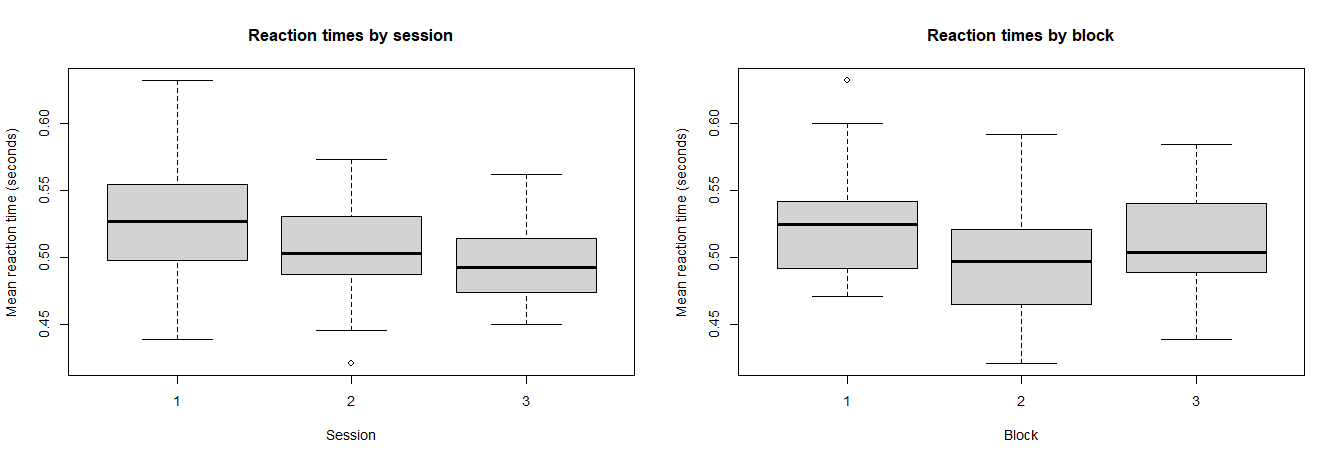
\includegraphics[width=0.9\linewidth]{Project plots/blocksession plots.png}
    \vspace{-0.5cm}
    \caption{Reaction times by Block and Session}
    \label{fig:blocksessiontimes}
\end{figure}


Based on Figure~\ref{fig:blocksessiontimes}, we introduced the planned blocking factors, \texttt{session} and \texttt{block}, to account for both day-to-day and within-day variation caused by uncontrollable sources of variation such as my concentration levels during testing, eyestrain from prolonged screen exposure, improvement from repeated reaction practise, etc.


\begin{lstlisting}[style=RStudioNonum]
MLR_BLOCK <- lm(mean_time ~ font_size + factor(font_colour) + factor(bg_colour) + factor(block), data = REACTION_TIMES_BEN)
MLR_SESSION <- lm(mean_time ~ font_size + factor(font_colour) + factor(bg_colour) + factor(session), data = REACTION_TIMES_BEN)
MLR_RBD <- lm(mean_time ~ font_size + factor(font_colour) + factor(bg_colour) + factor(session) + factor(block), data = REACTION_TIMES_BEN)
anova(MLR,MLR_RBD)
anova(MLR, MLR_BLOCK)
anova(MLR, MLR_SESSION)
anova(MLR_BLOCK, MLR_RBD)
anova(MLR_SESSION, MLR_RBD)
\end{lstlisting}
\rinline{anova(MLR,MLR_RBD)} returned a p-value of $1.36\cdot 10^{-8}$ which gives strong evidence to reject the null hypothesis that including both blocking factors didn't improve the model's fit to the data:
\begin{lstlisting}[style=RStudioNonum]
> anova(MLR,MLR_RBD)
Analysis of Variance Table

Model 1: mean_time ~ font_size + factor(font_colour) + factor(bg_colour)
Model 2: mean_time ~ font_size + factor(font_colour) + factor(bg_colour) + 
    factor(session) + factor(block)
  Res.Df      RSS Df Sum of Sq      F    Pr(>F)    
1    103 0.089311                                  
2     99 0.058422  4  0.030889 13.086 1.361e-08 ***

\end{lstlisting}

We also noted that by adding both blocking factors, the model $RSS$ was decreased by $34.6\%$:
\begin{lstlisting}[style=RStudioNonum]
> 1 - (anova(MLR_RBD)["Residuals", "Sum Sq"]/anova(MLR)["Residuals", "Sum Sq"])
[1] 0.3458574
\end{lstlisting}

\subsubsection{Interaction terms}\label{app:interactions}
Two-way interaction terms were evaluated by observing the Plots in Figure~\ref{fig:interactions}. Although only \texttt{font\_size}$\times$\texttt{font\_colour} appeared with noticeably non-parallel lines, model comparison tests were applied against the main effects model:
\begin{lstlisting}[style=RStudioNonum, escapeinside={(*@}{@*)}]
int_models=lm(mean_time~font_size (*@\plusorstar@*) font_colour (*@\plusorstar@*) bg_colour)
anova(MLR_RBD, int_models)
\end{lstlisting}
As expected only \texttt{font\_size}$\times$\texttt{font\_colour} showed a borderline interaction term with $p=0.0595$. Hence we rejected the inclusion of interaction terms in our model.
\begin{figure}[H]
    \centering
    \vspace{-0.2cm}
    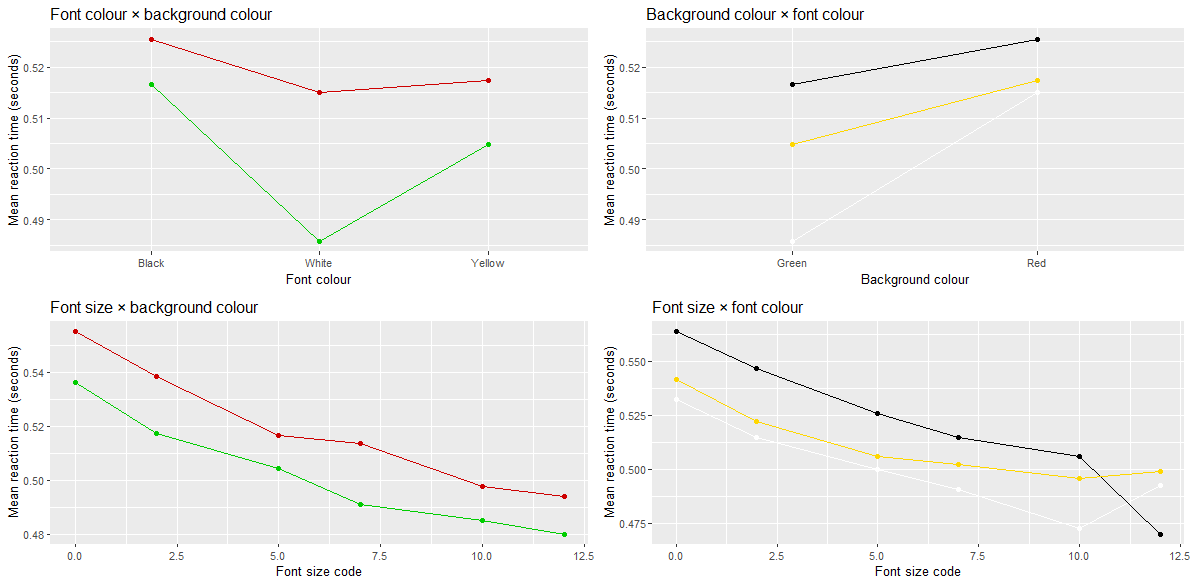
\includegraphics[width=0.72\linewidth]{Project plots/2x2interactions.png}
    \vspace{-0.3cm}
    \caption{Pairwise interaction plots}
    \label{fig:interactions}
\end{figure}
\newpage
\begin{lstlisting}[style=RStudioNonum]
> MLR_RBD_FS_FC <- lm(mean_time ~ font_size * factor(font_colour) + factor(bg_colour) + factor(session) + factor(block), data = REACTION_TIMES_BEN)
> anova(MLR_RBD, MLR_RBD_FS_FC)
Analysis of Variance Table

Model 1: mean_time ~ font_size + factor(font_colour) + factor(bg_colour) + 
    factor(session) + factor(block)
Model 2: mean_time ~ font_size * factor(font_colour) + factor(bg_colour) + 
    factor(session) + factor(block)
  Res.Df      RSS Df Sum of Sq      F  Pr(>F)  
1     99 0.058422                              
2     97 0.055112  2 0.0033107 2.9135 0.05905 .

> 1 - (anova(MLR_RBD_FS_FC)["Residuals", "Sum Sq"]/anova(MLR_RBD)["Residuals", "Sum Sq"])
[1] 0.05666789
\end{lstlisting}


It is noteworthy that removing the \texttt{block} nuisance factor from both models in the test, this interaction became significant with $p=0.033$. Hence we note that by allowing for variability in performance between each of the $3$ blocks of $12$ tests each session, the performance with black text specifically is not significantly different for larger font sizes. \newline

More complex interaction models (three way and nuisance interactions) were analysed, and rejected at the $5\%$ significance level, however, these have been omitted for brevity.

\subsubsection{Box Cox Transformations}\label{app:boxcox}

Despite diagnostic plots (Plot~\ref{plot:Plot4} and \ref{plot:Plot5}) demonstrating consistency with normality assumptions, a Box-Cox transformation check gave a parameter estimate very close to $0$, $\hat{\lambda} = -0.101$. Therefore, transformed models were observed under a log ($\lambda = 0)$ and lambda ($\lambda=-0.101$) Box-Cox transformation:



\begin{lstlisting}[style=RStudioNonum]
> bc <- boxcox(MLR_RBD, lambda = seq(-2, 2, length=100))
> lambda_hat <- bc$x[which.max(bc$y)]
> lambda_hat
[1] -0.1010101

MLR_RBD_BC_LOG <- lm(log(mean_time) ~ font_size + factor(font_colour) + factor(bg_colour) + factor(session) + factor(block), data = REACTION_TIMES_BEN)
MLR_RBD_BC_LAMBDA <- lm( ((mean_time^lambda_hat - 1) / lambda_hat) ~ font_size + factor(font_colour) + factor(bg_colour) + factor(session) + factor(block), data = REACTION_TIMES_BEN)
\end{lstlisting}
\begin{figure}[H]
    \centering
    \vspace{-0.7cm}
    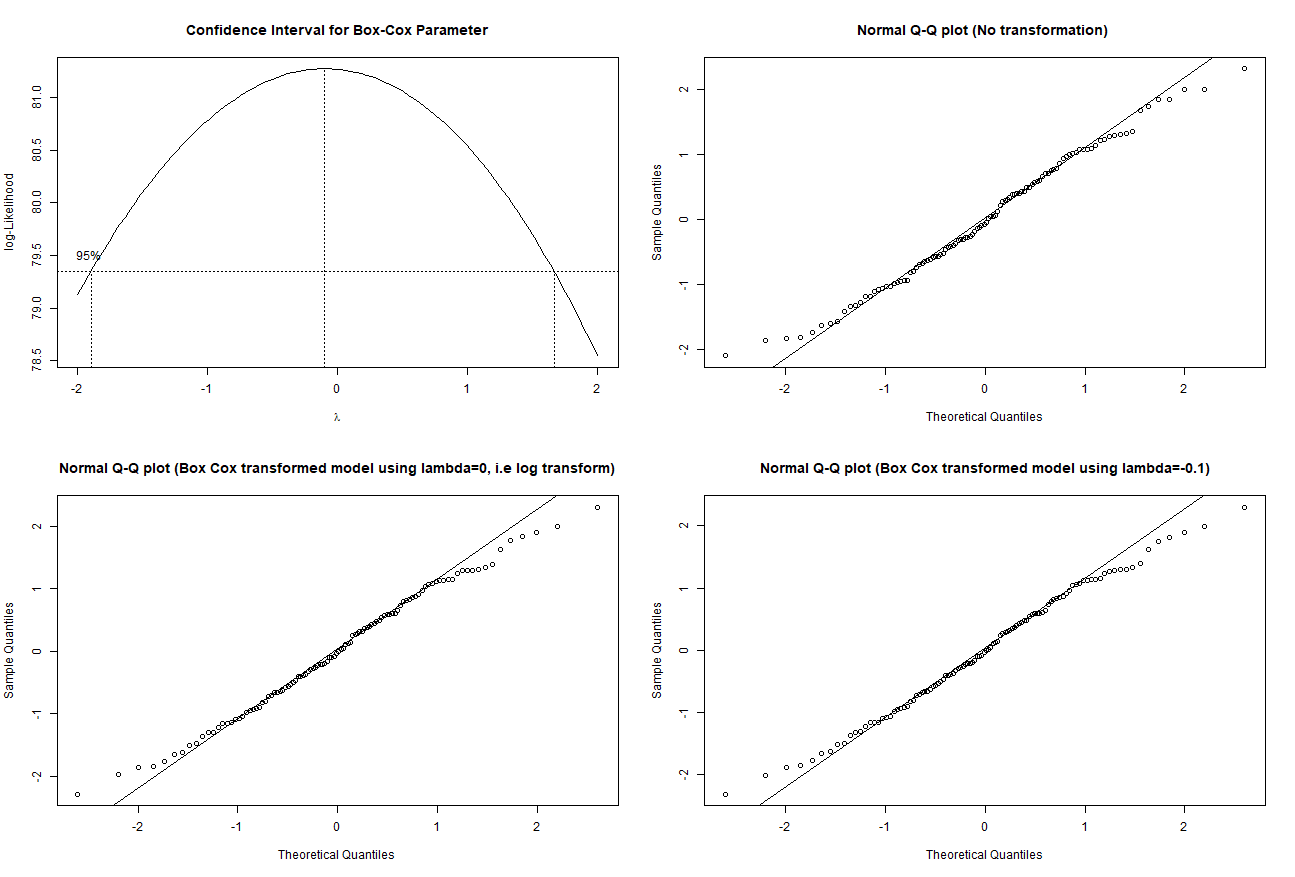
\includegraphics[width=0.66\linewidth]{Project plots/2by2boxcox.png}
    \vspace{-0.3cm}
    \caption{Box Cox Transformation Plots}
    \label{fig:boxcoxplots}
\end{figure}


Due to the enormous confidence interval seen in the first plot on Figure~\ref{fig:boxcoxplots}, and the lack of improvement in tail skewing in the bottom two plots on Figure~\ref{fig:boxcoxplots} relative to the second plot (no transformation), we rejected the need to apply a Box-Cox transformation.


\subsection{Final model summary}\label{app:model_summary_final}
\vspace{0.2cm}


\subsubsection{\texttt{MLR\_RBD} Model Summary and ANOVA}\label{app:model_summary}
\vspace{0.2cm}

Using the model summary and ANOVA outputs, we were able to compare key statistics such as the $R^2_{\text{adj}} = 0.5741$ and $RSS=0.058$ to understand the model's performance compared to alternative constructions we tried in the stepwise regression model selection process.

\begin{lstlisting}[style=RStudioNonum]
> MLR_RBD <- lm(mean_time ~ font_size + factor(font_colour) + factor(bg_colour) + factor(session) + factor(block), data = REACTION_TIMES_BEN)
> summary(MLR_RBD)

Call:
lm(formula = mean_time ~ font_size + factor(font_colour) + factor(bg_colour) + 
    factor(session) + factor(block), data = REACTION_TIMES_BEN)

            Estimate Std. Error t value Pr(>|t|)    
(Intercept)                0.5745008  0.0076750  74.853  < 2e-16 ***
font_size                 -0.0045930  0.0005584  -8.226 7.86e-13 ***
factor(font_colour)White  -0.0234953  0.0059835  -3.927 0.000159 ***
factor(font_colour)Yellow -0.0142337  0.0058476  -2.434 0.016720 *  
factor(bg_colour)Red       0.0175410  0.0046803   3.748 0.000300 ***
factor(session)2          -0.0231389  0.0057258  -4.041 0.000105 ***
factor(session)3          -0.0332778  0.0057258  -5.812 7.54e-08 ***
factor(block)2            -0.0228882  0.0058126  -3.938 0.000153 ***
factor(block)3            -0.0176060  0.0059633  -2.952 0.003938 ** 

Residual standard error: 0.02429 on 99 degrees of freedom
Multiple R-squared:  0.6059,	Adjusted R-squared:  0.5741 
F-statistic: 19.03 on 8 and 99 DF,  p-value: < 2.2e-16

> anova(MLR_RBD)

                    Df   Sum Sq  Mean Sq F value    Pr(>F)    
font_size            1 0.043449 0.043449 73.6270 1.347e-13 ***
factor(font_colour)  2 0.007795 0.003898  6.6046 0.0020302 ** 
factor(bg_colour)    1 0.007701 0.007701 13.0503 0.0004784 ***
factor(session)      2 0.020947 0.010474 17.7483 2.587e-07 ***
factor(block)        2 0.009942 0.004971  8.4233 0.0004185 ***
Residuals           99 0.058422 0.000590                      
\end{lstlisting}
\vspace{-0.3cm}
\subsubsection{Reaction Time Confidence Interval Over Font Size Range}\label{app:diff_CI}

\vspace{0.2cm}
Once we decided upon using \rinline{MLR_RBD}, the \rinline{emmeans} package was used to calculate the confidence interval for the difference between the maximum ($12$) and minimum ($0$) font sizes, averaged over all other model factors:
\begin{lstlisting}[style=RStudioNonum]
> library(emmeans)
> MLR_RBD <- lm(mean_time ~ font_size + factor(font_colour) + factor(bg_colour) + factor(session) + factor(block), data = REACTION_TIMES_BEN)
> confint(contrast(emmeans(MLR_RBD, ~ font_size, at = list(font_size = c(0, 12))), method = "pairwise"))
 
 contrast                 estimate     SE df lower.CL upper.CL
 font_size0 - font_size12   0.0551 0.0067 99   0.0418   0.0684
Results are averaged over the levels of: font_colour, background_colour, session, block 
Confidence level used: 0.95  
\end{lstlisting}

Hence, by defining $\Delta$ as the difference in expected mean reaction times between font size $0$ and $12$, under our model \rinline{MLR_RBD}, averaged over font and background colour, session and block:\\$\Delta := \mathbb{E}_{\text{MLR\_RBD}}\left(\texttt{mean\_time} \mid \texttt{font\_size}=0\right)
        - \mathbb{E}_{\text{MLR\_RBD}}\left(\texttt{mean\_time} \mid \texttt{font\_size}=12\right)$, we have the estimate $\widehat{\Delta} = 0.0551$ with a $95\%$ confidence interval of $\Delta \in (0.0418, 0.0684)$.

\subsubsection{Linear contrasts}\label{app:contrasts}
Linear contrasts were used to determine whether there existed significant differences in pairwise comparisons of the main effects of font and background colours.

\begin{lstlisting}[style=RStudioNonum]
library(emmeans)
> pairs(emmeans(MLR_RBD, ~ bg_colour))
 contrast    estimate      SE df t.ratio p.value
 Green - Red  -0.0175 0.00468 99  -3.748  0.0003

Results are averaged over the levels of: font_colour, session, block 
> pairs(emmeans(MLR_RBD, ~ font_colour))
 contrast       estimate      SE df t.ratio p.value
 Black - White   0.02350 0.00598 99   3.927  0.0005
 Black - Yellow  0.01423 0.00585 99   2.434  0.0437
 White - Yellow -0.00926 0.00583 99  -1.590  0.2548

Results are averaged over the levels of: bg_colour, session, block
\end{lstlisting}

These results support our project summary statistics that black is significantly slower than both white and yellow, whereas, white and yellow do not have significantly different reaction times. What's more, reaction times on green backgrounds are significantly faster than on red backgrounds.


\subsubsection{Diagnostic plots}\label{app:diagnostics}
Plots~\ref{plot:Plot4} and \ref{plot:Plot5}, combined with Figure~\ref{fig:standresds} below demonstrate the fitted values and test data indices of \rinline{MLR\_RBD} plotted against its standardised residuals. The apparent random scatter and constant variance indicate that the normality model assumptions are valid.

\begin{figure}[H]
    \centering
    \vspace{-0.5cm}
    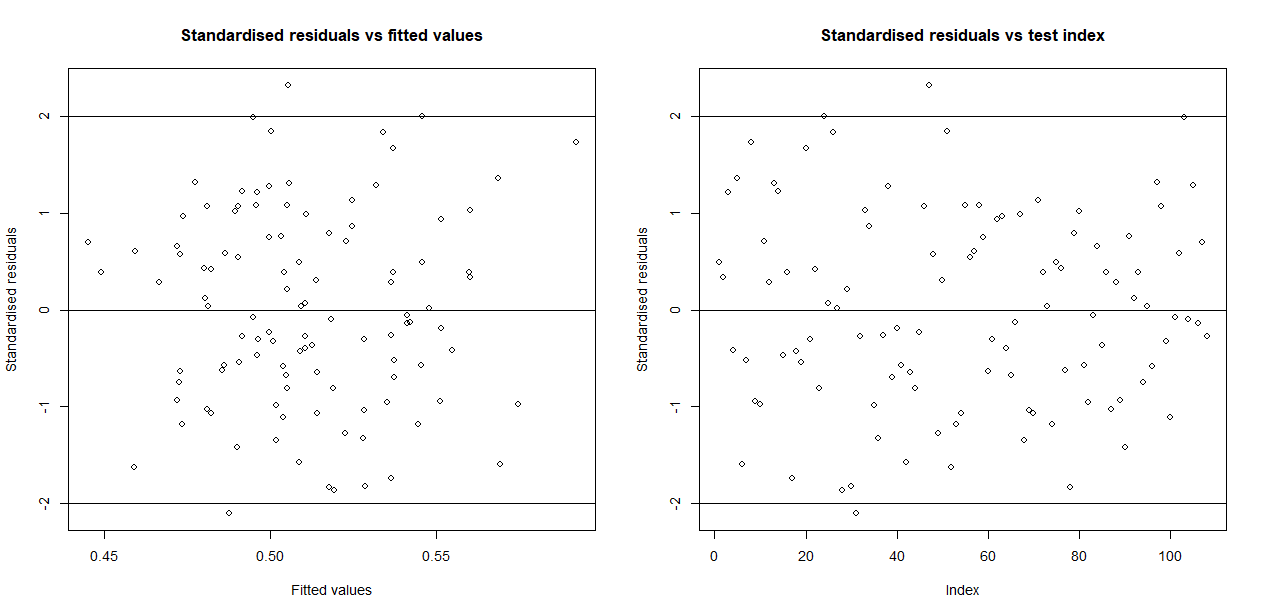
\includegraphics[width=0.8\linewidth]{Project plots/standardisedresds.png}
    \vspace{-0.4cm}
    \caption{\texttt{MLR\_RBD} standardised residuals vs fitted values, and test data indices}
    \label{fig:standresds}
\end{figure}


Computing the proportion of the standardised residuals in $(-Z_{0.975}, Z_{0.975})$ we have:
\begin{lstlisting}[style=RStudioNonum]
> STD_RS <- rstandard(MLR_RBD)
> mean(abs(STD_RS) <= 1.96)
[1] 0.962963
\end{lstlisting}

We can see that this output is very close to $0.95$ which is what we would expect under $\mathcal{N}(0,1)$, hence validating our visual observation of the standardised residuals adherence to the assumed variance of $1$.\newline

\hrulefill


\end{document}
